\section{Auswertung} \label{sec:auswertung}

\subsection{Modell} \label{subsec:modell}

Für die Berechnung der potentiellen Energie benützen wir das Modell Park Avenue 432, eines der höchsten reinen Wohnhochhäusern auf der Welt. Die stolze Höhe und der über das ganze Gebäude gleichbleibende quadratische Grundriss sind ideal für unsere Berechnungen. Für die Wassermengenberechnung stützen wir uns auf die Angaben des durchschnittlichen Wasserverbrauch in Amerika pro Person und Tag: 314\si{L}. \cite{waterUsAmerica}

\begin{figure} [H]
	\centering
	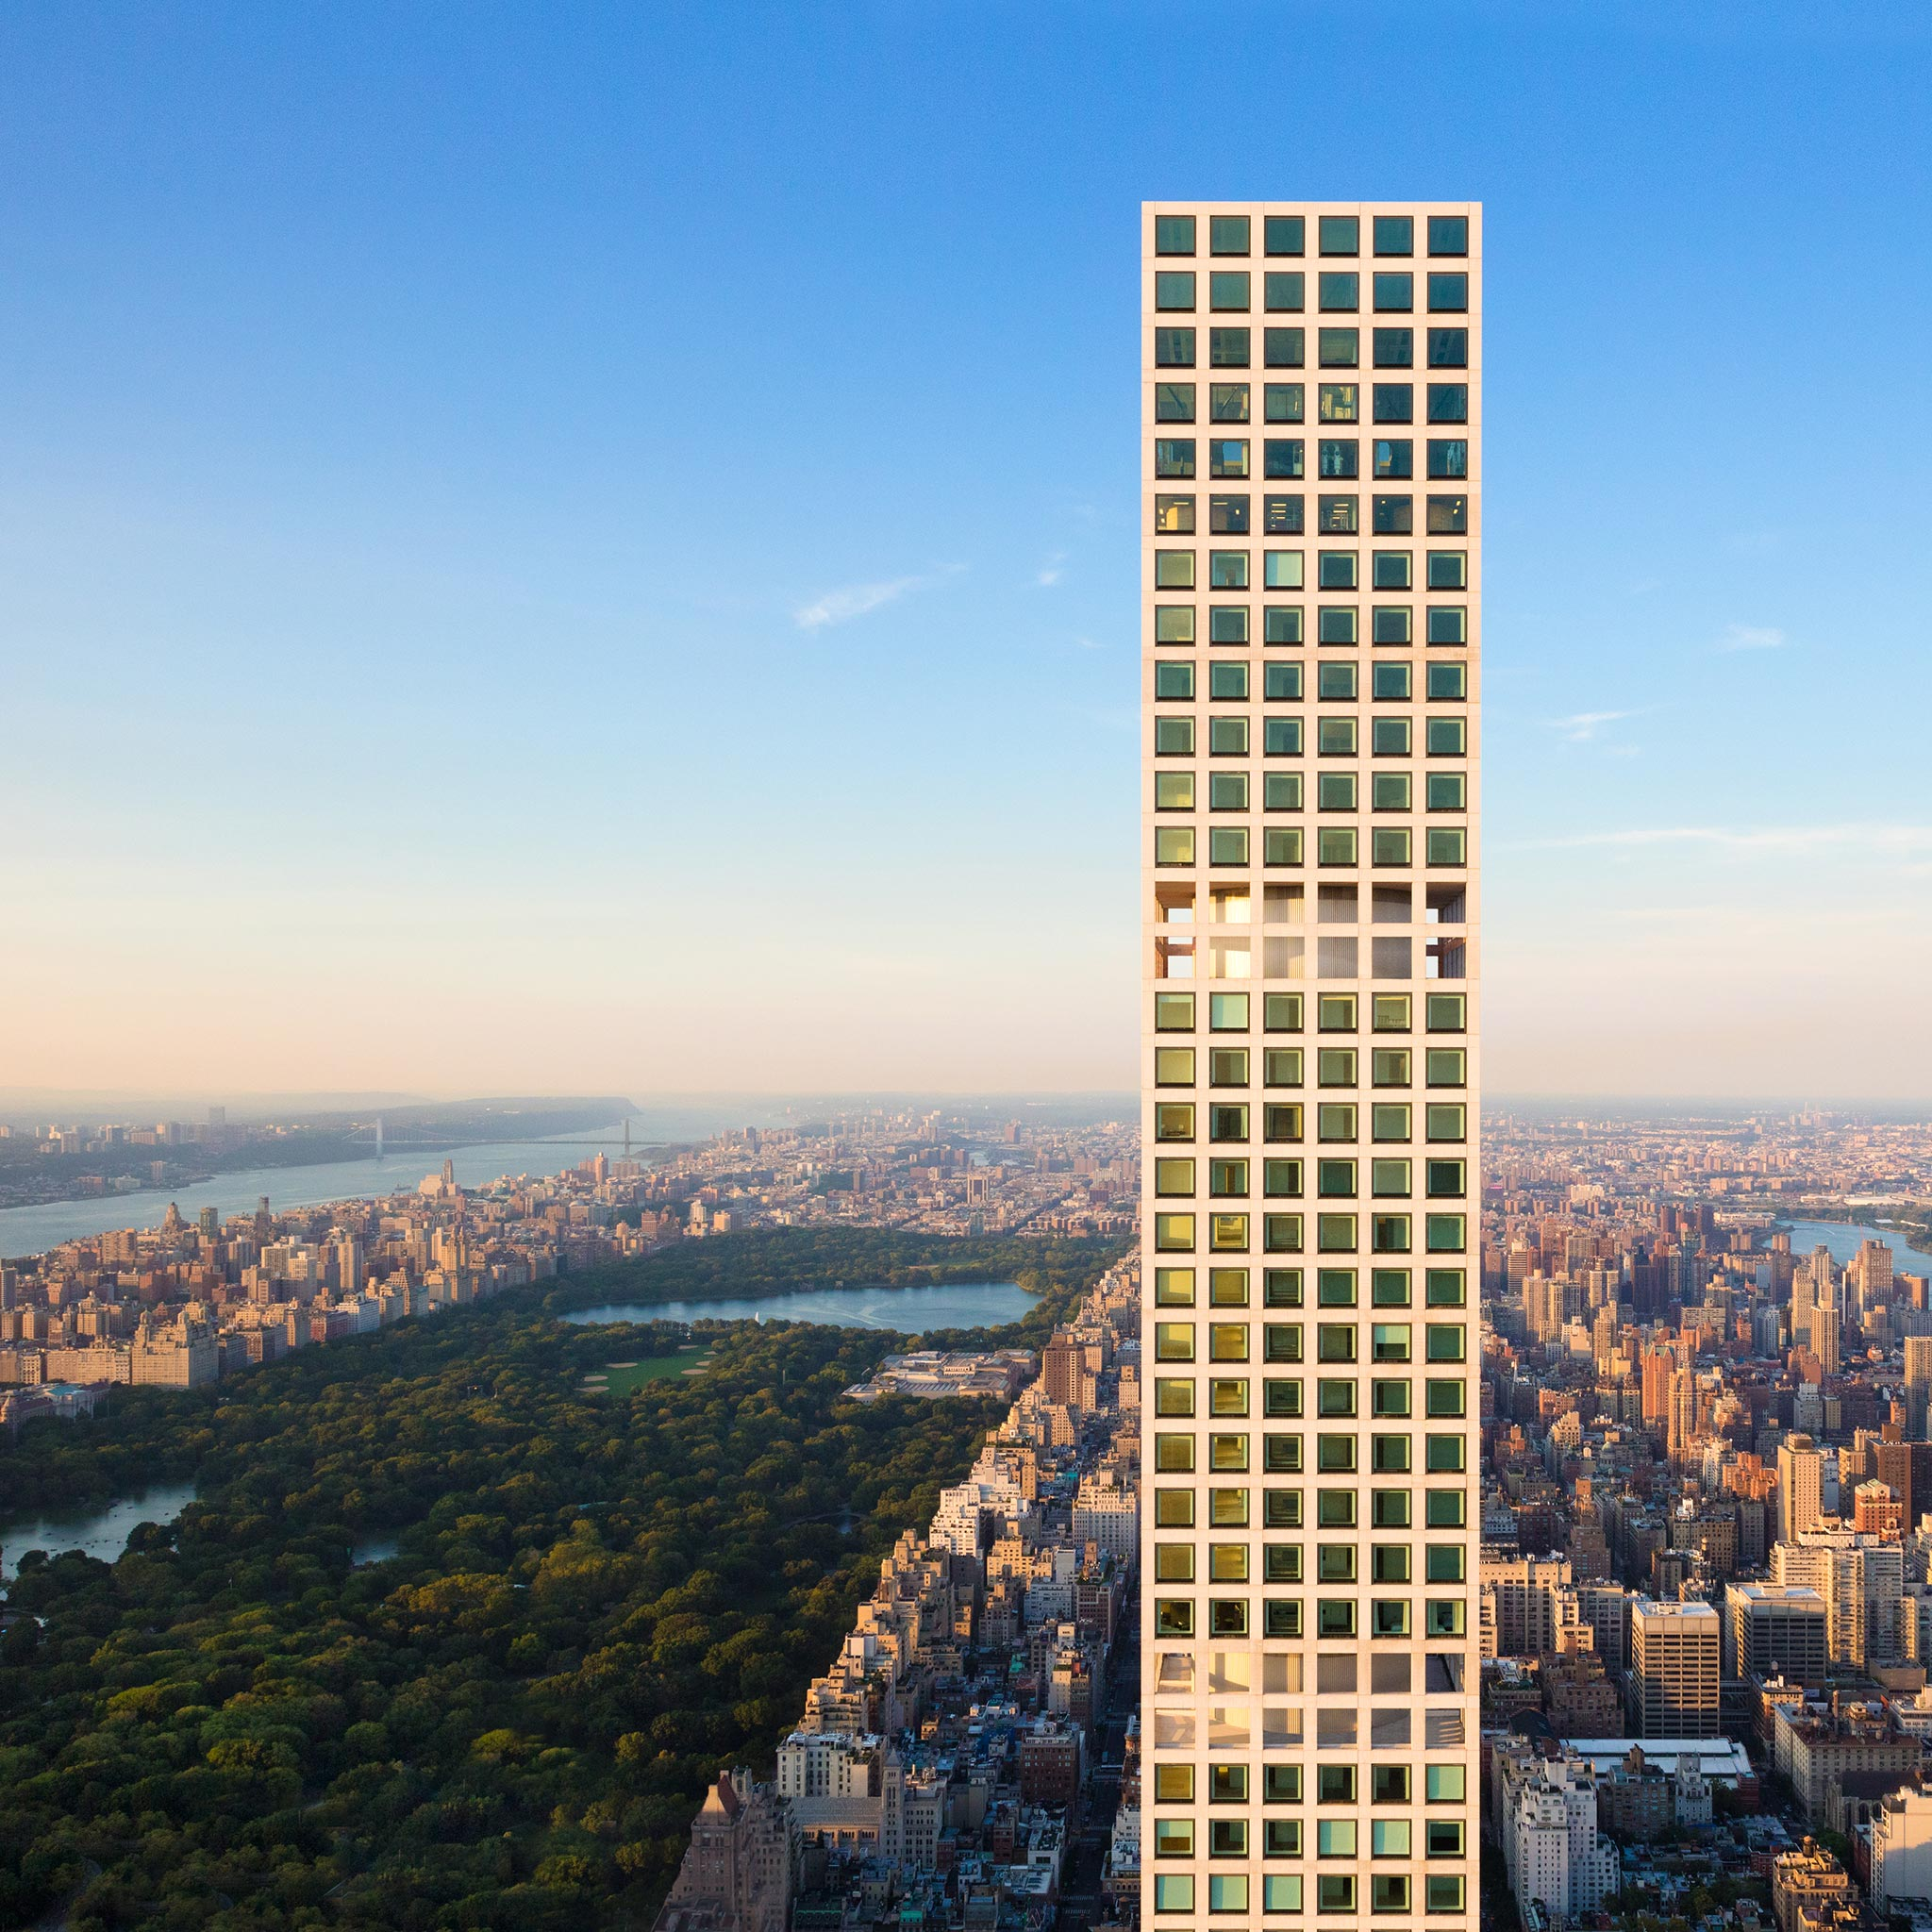
\includegraphics[width=12cm]{parkAvenue.jpg}
	\caption{Park Avenue 432 \cite{432_Park_Avenue}}
	\label{fig:Park_Avenue_432}
\end{figure}

\begin{table}[H]
\centering
\begin{tabular}{ll}
Name:				&Park Avenue 432\\
Höhe: 				&426m\\          
Etagen:				&84 Obergeschosse, 1 Erdgeschosse, 3 Untergeschosse\\
Etagenhöhe:			&4.72m\\
Hoechste Etage:		&392.1m\\
Wohnungen:			&146\\
Speziell:			&alle 12 Etagen 2 Etagen leer\\           
\end{tabular}
\end{table}

\newpage

\subsection{Energieberechnung} \label{subsec:energieberechnung}

Die Endgeschwindigkeit des Abwassers kann mit folgender Formel berechnet werden:
\begin{center}
\[
	v = \sqrt{2 \cdot g \cdot h}
\]
\end{center}

Die Einheit der Geschwindigkeit \(v\) ist \si{m/s}, das Schwerefeld \(g\) auf der Erde besitzt den Wert 9.81~\si{N/kg}, und die Höhe \(h\) hat die Einheit \si{m}.

\bigskip

Die Energie, die gewonnen werden kann, wird mit folgender Formel berrechnet:

\begin{center}
\[
	E =\frac 12\ \cdot m \cdot v^2
\]
\end{center}

Die Energie \(E\) hat die Einheit \si{J}, die Einheit der Geschwindigkeit \(v\) ist \si{m/s}, und die Masse \(m\) hat die Einheit \si{kg}

\bigskip

Um die Leistung in \si{kWh} zu erhalten wird forlgende Formel verwendet:

\begin{center}
\[
	P = \frac{E \cdot \eta}{3.6\si{MJ}}
\]
\end{center}

Die Leistung \(P\) hat die Einheit \si{W} und der Wirkungsgrad \(\eta\) besitzt keine Einheit.

\newpage

Mit diesen mathematischen Grundlagen kann nun von jedem Grobkonzept die Leistung anhand des Modellhochhauses berechnet werden. Für die Berchnungen wird angenommen, dass pro Wohnung 2.5 Personen leben und diese einen Durchschnittsverbrauch pro Tag von 785\si{L} haben. Bei 146 Wohnungen und 74 Nutzbaren Etagen leben 5 Personen pro Etage. Es wird somit 1570\si{L} pro Etage pro Tag verbraucht. Im Anhang befindet sich das vereinfachte Modell (\ref{fig:VereinfachtesModel} \nameref{fig:VereinfachtesModel}) des Hochhauses, von dem die Berechnungen ausgehen. Das gesamte Hochhaus wird zur Vereinfachung in 6 Blöcke unterteilt. Dies ist, zusammen mit einer Legende für die benutzten Symbole, in der Abbildung \ref{fig:EinteilungBloecke} \nameref{fig:EinteilungBloecke} ersichtlich.

\bigskip

\begin{figure} [H]
	\centering
	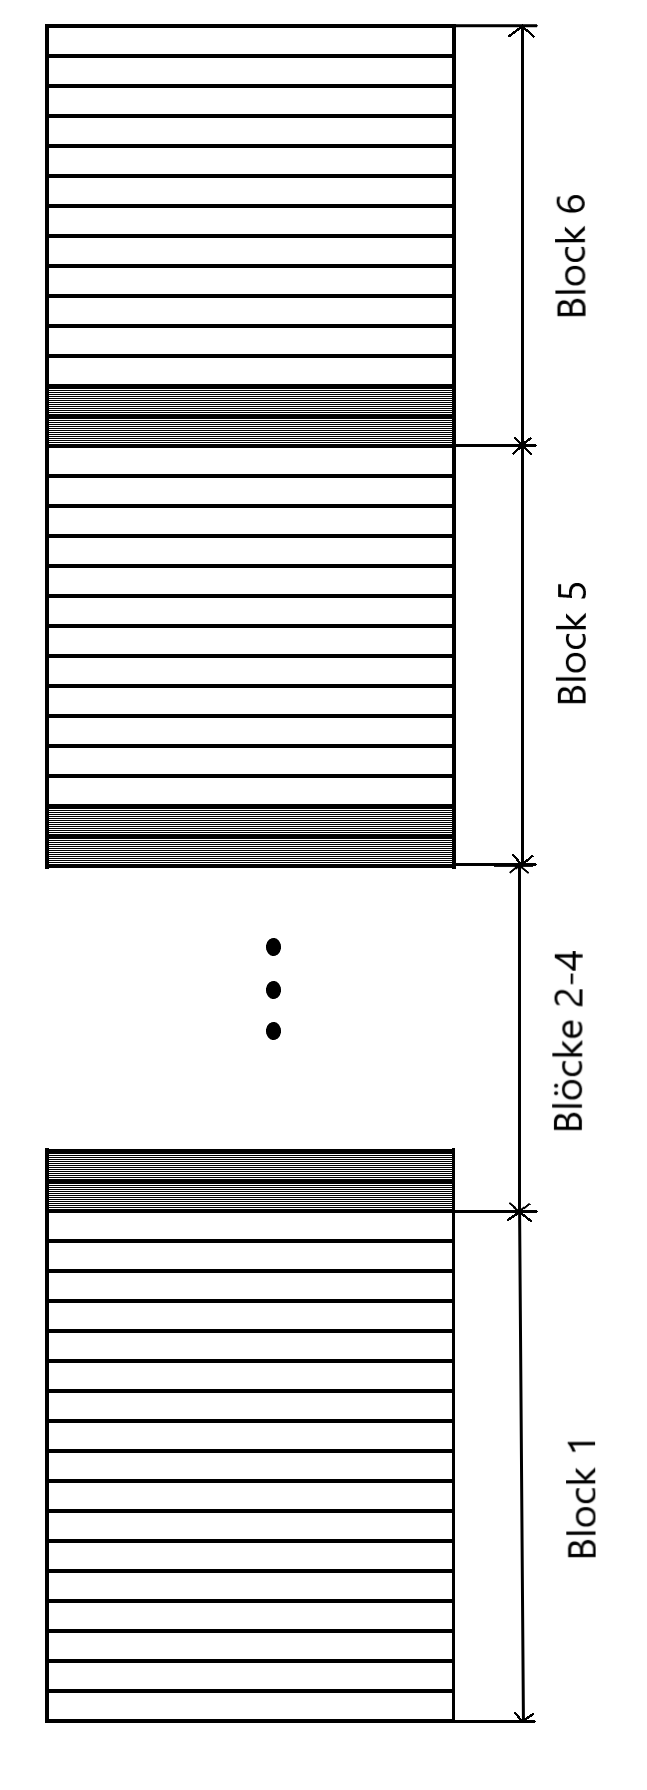
\includegraphics[width=11cm]{EinteilungBloecke.png}
	\caption{Blockeinteilung des Hochhauses}
	\label{fig:EinteilungBloecke}
\end{figure}

\newpage

\paragraph{Grobkonzept 1} 

Im Grobkonzept 1 wird die Geschwindigkeit des Abwassers ausgenutzt. Wie bereits im Recherchedokument \cite{recherchedokument} berechnet, wird das Wasser ab ca. 10m nicht mehr merklich schneller. Um möglichst viel Energie zu erzeugen wird in jeder zweiten Etage, also alle 9.44\si{m} ein kleines Wasserrad eingebaut. Ingesamt werden 43 Wasserräder eingebaut. Dies ist in der Abbildung \ref{fig:PrinzipGrobkonzept1} \nameref{fig:PrinzipGrobkonzept1} ersichtlich. Die Geschwindigkeit des Abwassers beträgt bei einer Höhe von zwei Etagen 8.5\si{m/s} und bei einer Etage 6.5\si{m/s}

\begin{figure} [H]
	\centering
	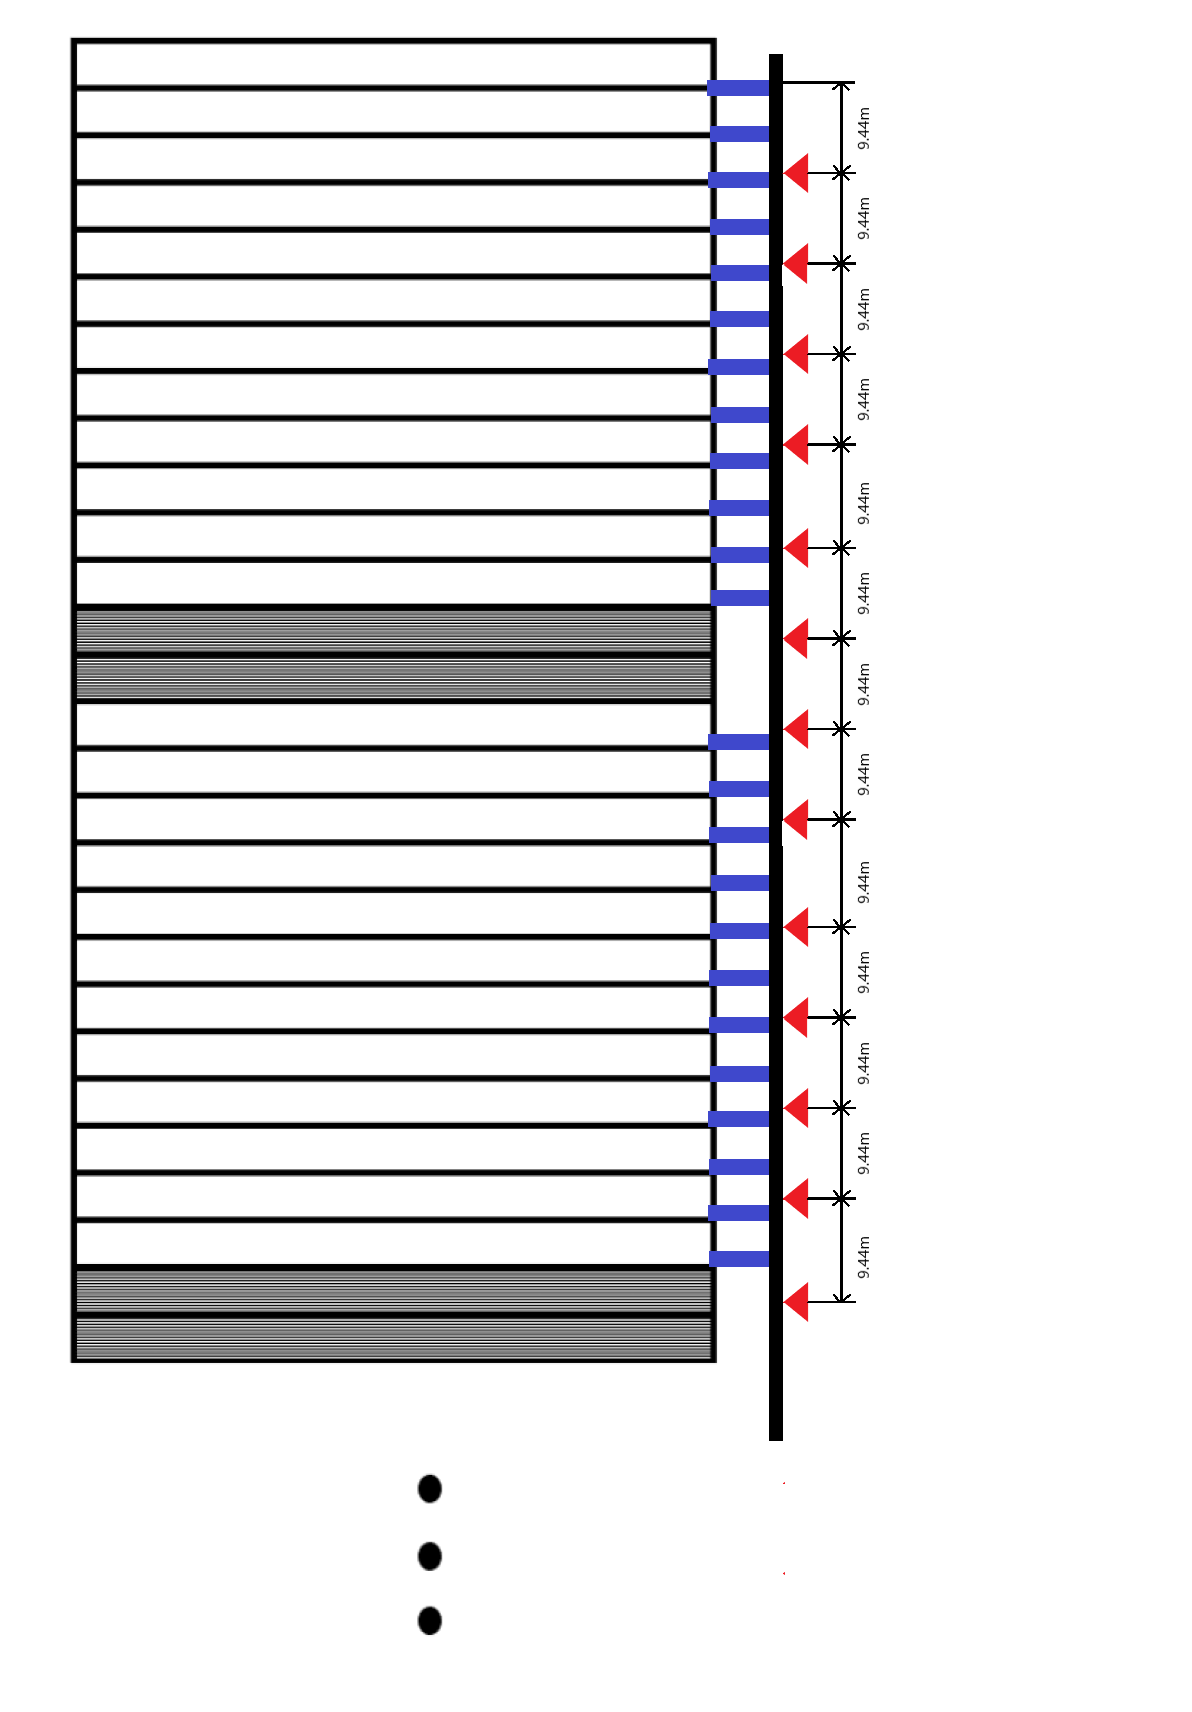
\includegraphics[width=9cm]{PrinzipGrobkonzept1.png}
	\caption{Prinzip Grobkonzep 1}
	\label{fig:PrinzipGrobkonzept1}
\end{figure}

Mit diesem Konzept wird insgesamt 21.5\si{kWh} pro Tag gewonnen, dies entspricht bei Stromkosten von 20\si{rp} einem Wert von 4.30\si{Fr}. Die Leistungsberechnungen sind im Anhang \ref{fig:BerechnungGrobkonzept1} \nameref{fig:BerechnungGrobkonzept1} zu finden.

\newpage

\paragraph{Grobkonzept 2}

Im Grobkonzept 2 wird die Geschwindigkeit des Abwassers ausgenutzt. Um den Luftwiderstand zu eliminieren, werden nun Druckleitungen eingebaut, die komplett mit Abwasser gefüllt werden. So kann eine grössere Geschwindigkeit erreicht werden. In den unbenutzen Etagen wird das Wasser gesammelt und mit einer Druckleitung bis zur Turbine ganz unten geführt. Dies ist in der Abbildung \ref{fig:PrinzipGrobkonzept2} \nameref{fig:PrinzipGrobkonzept2} ersichtlich.

\begin{figure} [H]
	\centering
	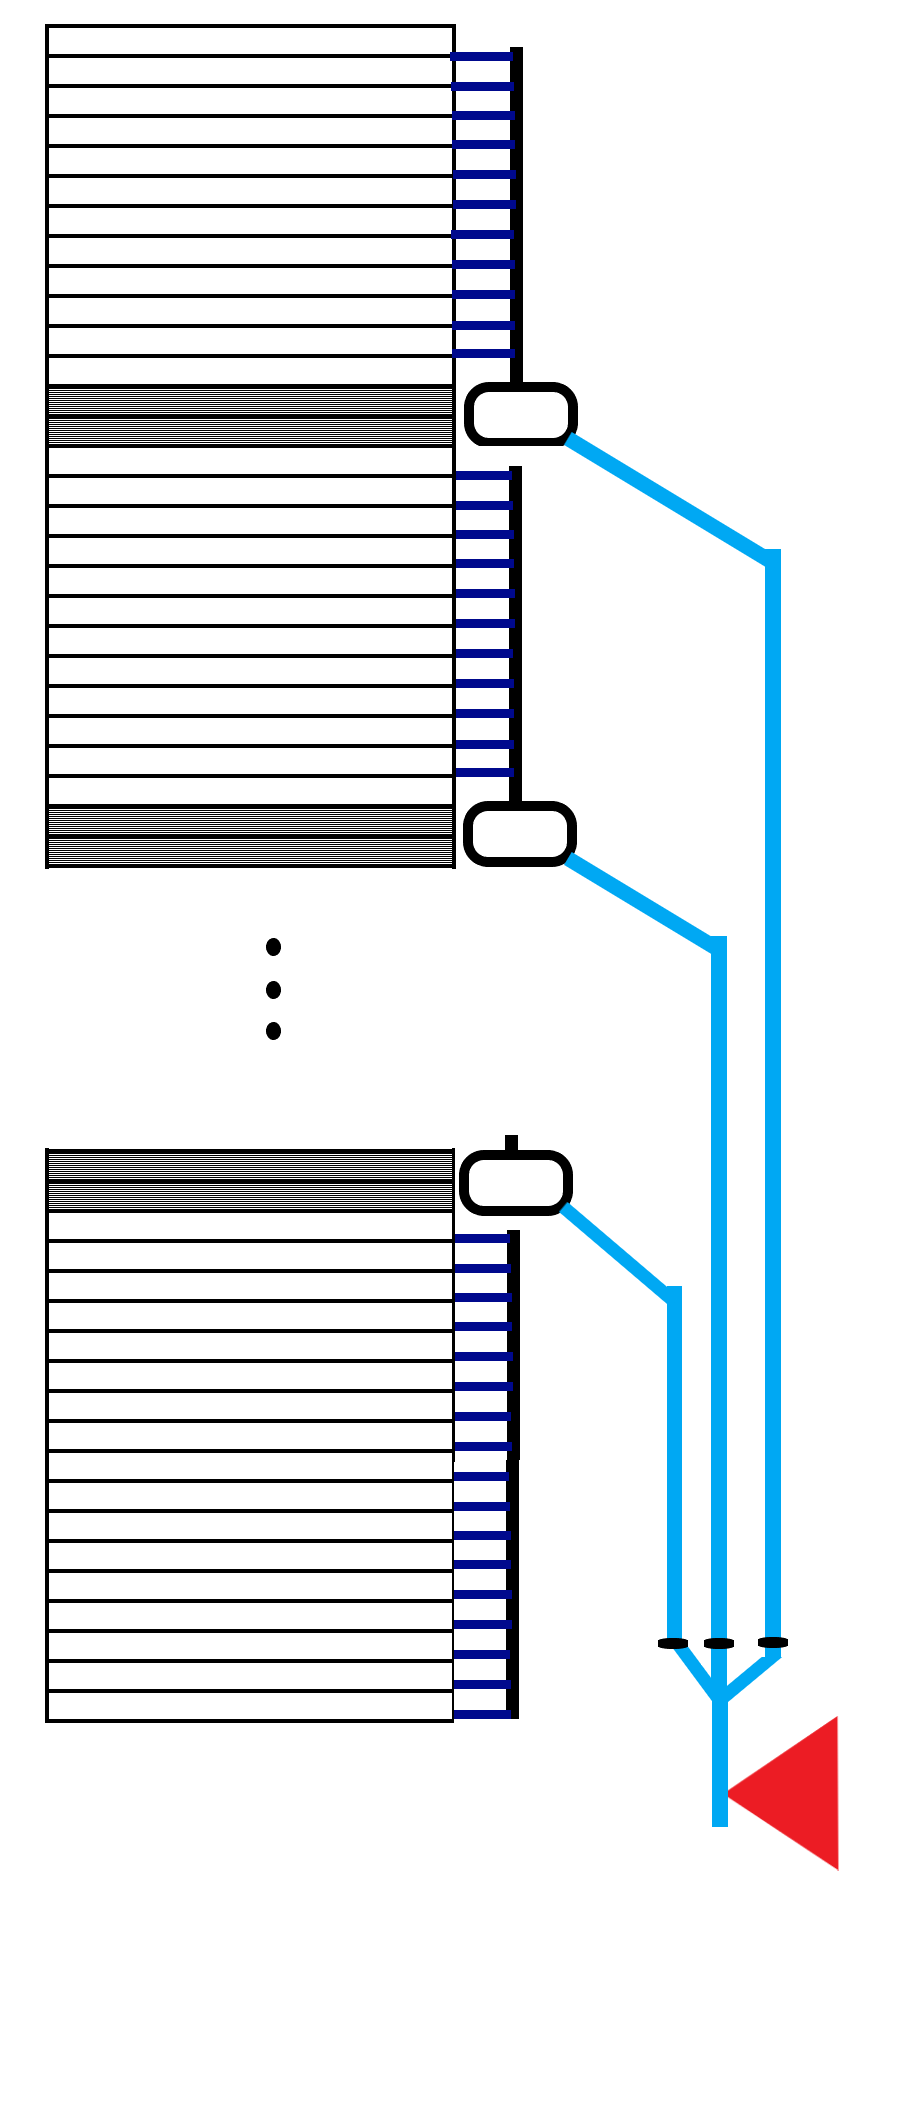
\includegraphics[width=7cm]{PrinzipGrobkonzept2.png}
	\caption{Prinzip Grobkonzep 2}
	\label{fig:PrinzipGrobkonzept2}
\end{figure}

Mit diesem Konzept wird ingesamt 44.59\si{kWh} pro Tag gewonnen, dies entspricht bei Stromkosten von 20\si{rp} einem Wert von 8.92\si{Fr}. Die Leistungsberechnungen sind im Anhang \ref{fig:BerechnungGrobkonzept2} \nameref{fig:BerechnungGrobkonzept2} zu finden.

\newpage

\paragraph{Grobkonzept 3}

Im Grobkonzept 3 wird die Geschwindigkeit des Abwassers ausgenutzt. Auch hier werden Druckleitungen eingebaut, um den Luftwiderstand zu eliminieren. So kann eine grössere Geschwindigkeit erreicht werden. In den unbenutzen Etagen wird das Wasser gesammelt und mit einer Druckleitung bis zur Turbine vor dem nächsten Tank geführt. Dies ist in der Abbildung \ref{fig:PrinzipGrobkonzept3} \nameref{fig:PrinzipGrobkonzept3} ersichtlich. 

\begin{figure} [H]
	\centering
	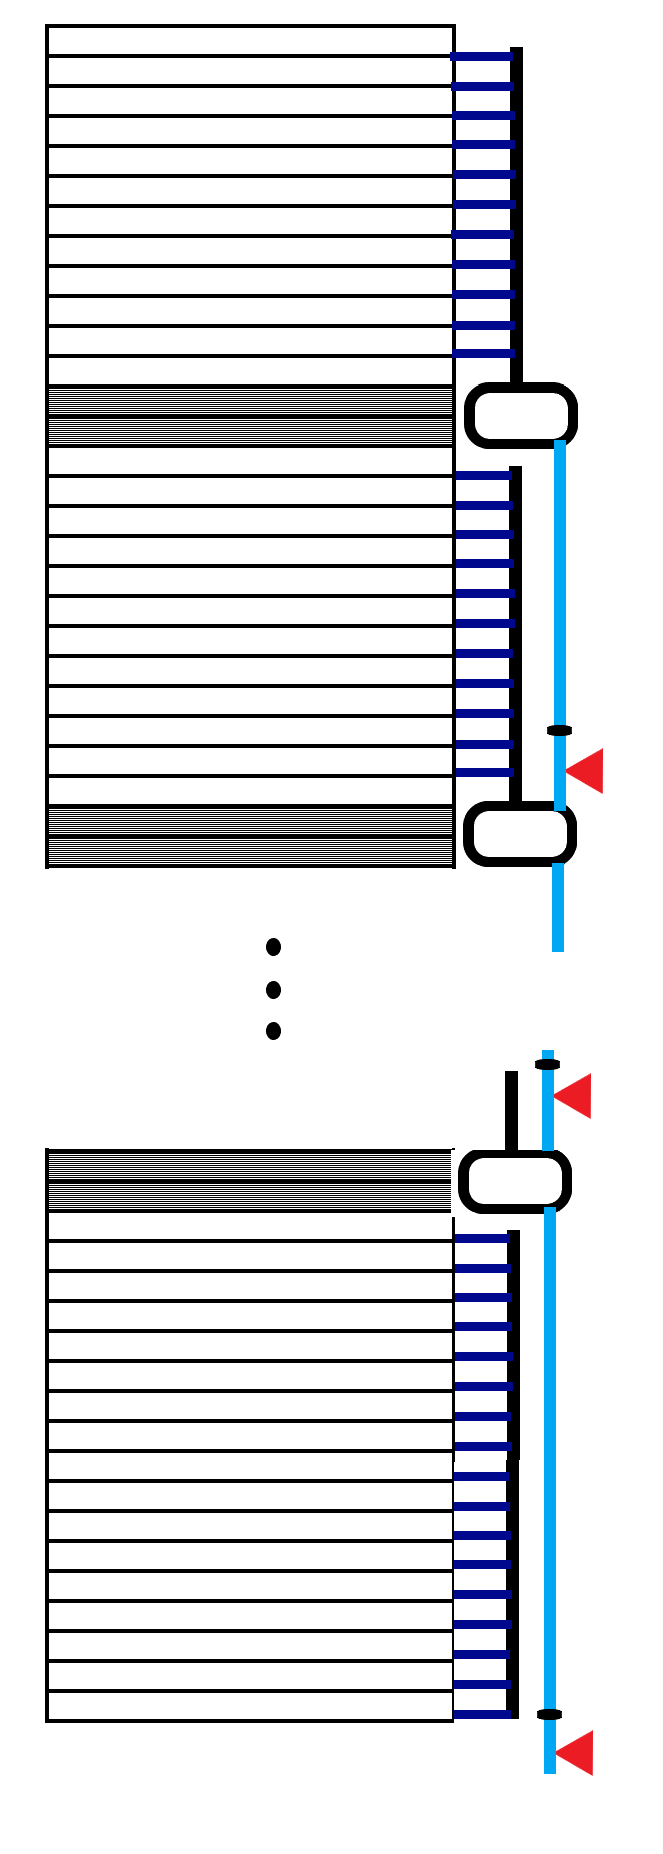
\includegraphics[width=6cm]{PrinzipGrobkonzept3.png}
	\caption{Prinzip Grobkonzep 3}
	\label{fig:PrinzipGrobkonzept3}
\end{figure}

Mit diesem Konzept wird ingesamt 42.62\si{kWh} pro Tag gewonnen, dies entspricht bei Stromkosten von 20\si{rp} einem Wert von 8.53\si{Fr}. Die Leistungsberechnungen sind im Anhang \ref{fig:BerechnungGrobkonzept3} \nameref{fig:BerechnungGrobkonzept3} zu finden.

\newpage

\paragraph{Grobkonzept 4}

Im Grobkonzept 4 wird die potenzielle Energie des Abwassers ausgenutzt. Damit die Wasserlifte nicht zu lang werden, werden diese Blockweise verbaut. Dies ist in der Abbildung \ref{fig:PrinzipGrobkonzept4} \nameref{fig:PrinzipGrobkonzept4} ersichtlich. Die obersten 5 Abschnitte bestehen aus 12 bewohnten und 2 ungenutzten Etagen. Der unterste Block besteht aus 16 bewohnten Etagen. Somit haben 5 Lifte eine Länge von 66.08\si{m} und der unterste Lift eine Länge von 80.24\si{m}

\begin{figure} [H]
	\centering
	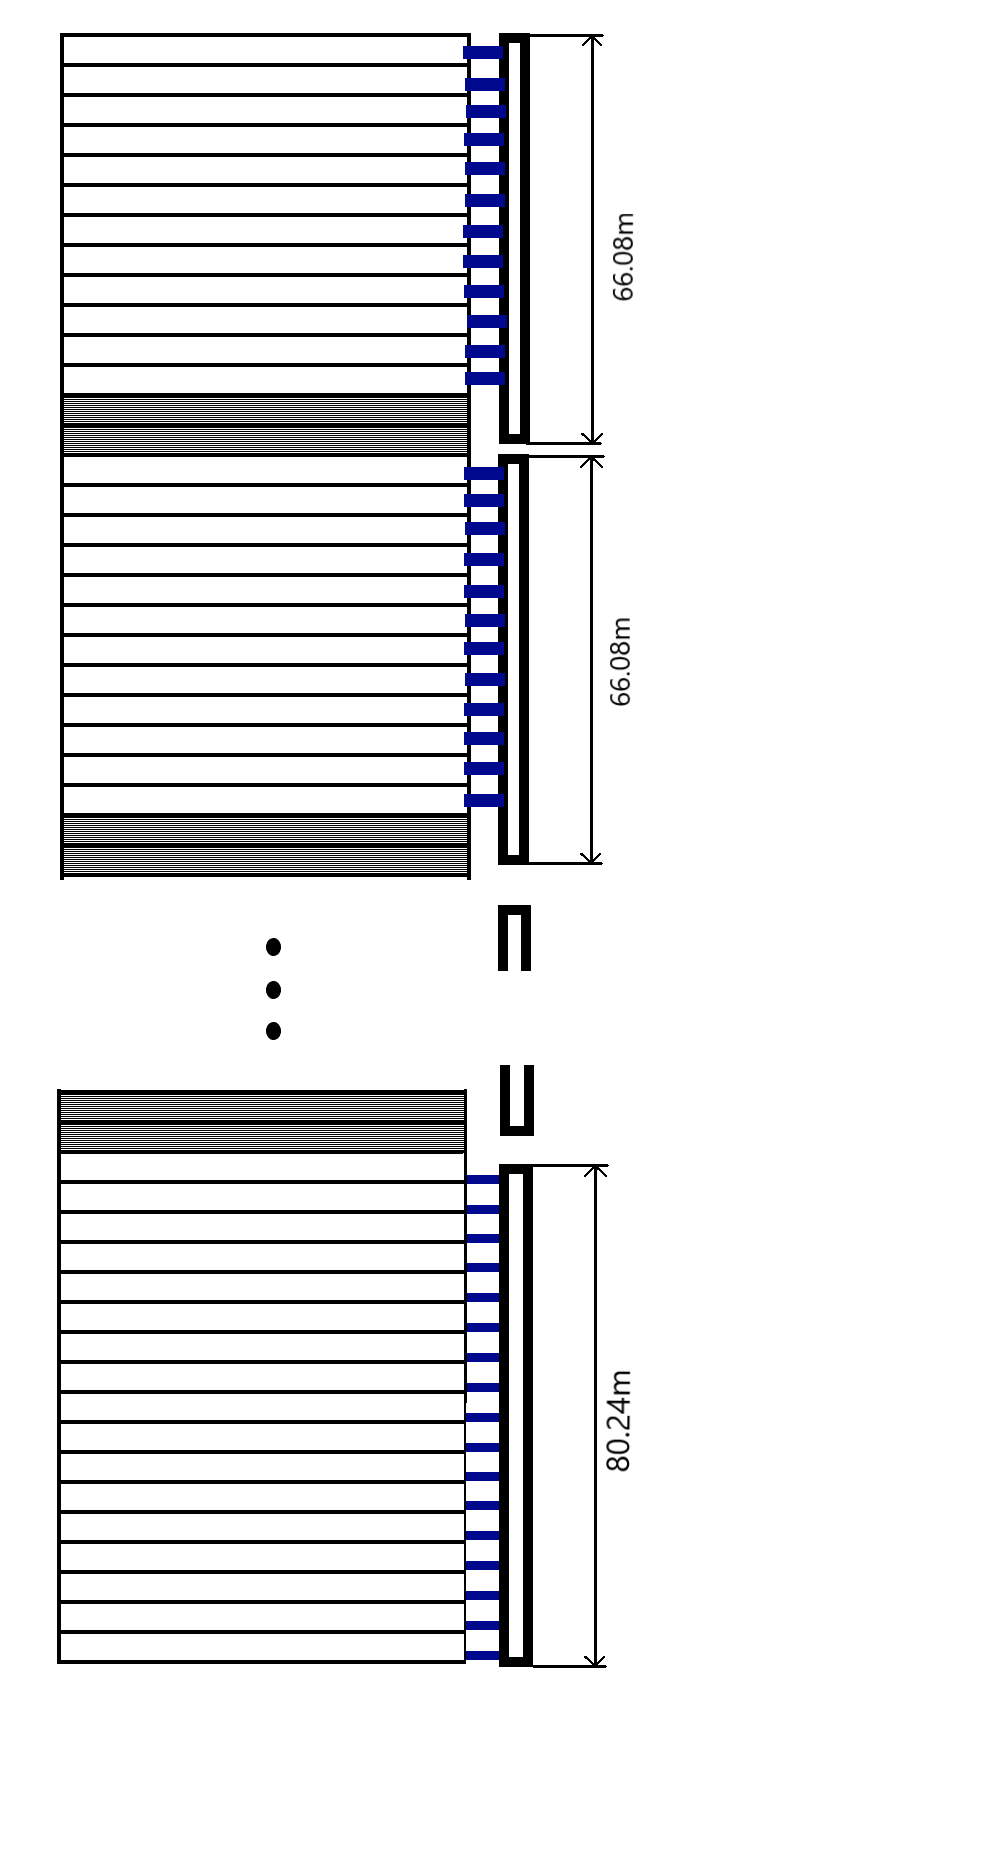
\includegraphics[width=8cm]{PrinzipGrobkonzept4.png}
	\caption{Prinzip Grobkonzep 4}
	\label{fig:PrinzipGrobkonzept4}
\end{figure}

Mit diesem Konzept wird ingesamt 53.08\si{kWh} pro Tag gewonnen, dies entspricht bei Stromkosten von 20\si{rp} einem Wert von 10.62\si{Fr}. Die Leistungsberechnungen sind im Anhang \ref{fig:BerechnungGrobkonzept4} \nameref{fig:BerechnungGrobkonzept4} zu finden.

\newpage
\subsection{Nutzwertanalyse} \label{subsec:nutzwertanlyse}
\renewcommand{\arraystretch}{1.5}
\newcommand{\vtcl}[1]{\rotatebox{90}{#1}}%\newcommand{\vtcl}[1]{\rotatebox{90}{\textbf{#1}}}
%\newcommand{\diagL}[1]{\diagbox{\hspace{#1}}{\hspace{#1}}}
Das Team konnte durch folgende Nutzwertanalyse bestimmen, welches Grobkonzept am ehesten in Fage kommt.
%\begin{table}[H]
%\small
%\begin{tabular}{l|llll|rr}
%&\vtcl{1.1. Wirkungsgrad}&\vtcl{1.2. Leistung}&\vtcl{1.3. Komplexität}&\vtcl{2.1. Platzbedarf}&\vtcl{Total}&\vtcl{Prozent}\\%\vtcl{2.1. Verstopfungsgefahr}&\vtcl{2.2. Platzbedarf}&\vtcl{2.3. Wartung}&\vtcl{Total}&\vtcl{Prozent}\\
%\hline
%1.1. Wirkungsgrad		&\cellcolor{black}	&0.5					&0.5					&0.5					&2.		&13\%\\
%1.2. Leistung			&0.5					&\cellcolor{black}	&1					&1					&4.5		&30\%\\
%1.3. Komplexität			&0.5					&0					&\cellcolor{black}	&0					&1.0		&6.5\%\\
%2.1. Verstopfungsgefahr	&1					&0					&1					&\cellcolor{black}	&0					&1					&3		&20\%\\
%2.1. Platzbedarf			&0.5					&0					&1					&\cellcolor{black}	&3.5		&24\%\\
%2.3. Wartung			&0.5					&0					&0.5					&0					&0					&\cellcolor{black}	&1.0		&6.5\%\\
%\hline
%\multicolumn{7}{c}{}&\textbf{15}&\textbf{100}\%\\
%\end{tabular}
%\end{table}
%\begin{scriptsize}
%Zeile-Kriterium ist wichtiger als Spalten-Kriterium 1\\
%Zeile-Kriterium ist gleich wichtig wie Spalten-Kriteriium 0.5\\
%Zeile-Kriterum ist weniger wichtig wie Spalternkriterium 0\\
%\end{scriptsize}
\newcolumntype{C}[1]{>{\centering}p{#1}}


\renewcommand\arraystretch{1.5}
\newcolumntype{R}[1]{>{\HY\RaggedLeft}p{#1}}
\newcolumntype{L}[1]{>{\HY\RaggedRight}p{#1}}
\renewcommand{\vtcl}[1]{\rotatebox{90}{\textbf{#1}}}
\begin{table}[H]
\caption{Nutzwertanalyse}\label{tab:nutzwertanalyse}
\small
\rotatebox{90}{
%|R{1.2cm}R{0.4cm}R{0.8cm} \scriptsize
%|R{1cm}R{0.2cm}R{0.5cm} \tiny
\begin{tabular}{lrR{0.8cm}|rrr|rrr|rrr|rrr|}%|R{1cm}R{0.5cm}R{0.8cm}
&&Max&\multicolumn{3}{c}{Grobkonzept 1}&\multicolumn{3}{c}{Grobkonzept 2}&\multicolumn{3}{c}{Grobkonzept 3}&\multicolumn{3}{c}{Grobkonzept 4}\\
\textbf{Zielkriterium}&\vtcl{Gewichtung}&\vtcl{Nutzwert}&\vtcl{Wert}&\vtcl{Erfüllungsgrad}&\vtcl{Nutzwert}&\vtcl{Wert}&\vtcl{Erfüllungsgrad}&\vtcl{Nutzwert}&\vtcl{Wert}&\vtcl{Erfüllungsgrad}&\vtcl{Nutzwert}&\vtcl{Wert}&\vtcl{Erfüllungsgrad}&\vtcl{Nutzwert}\\
\hline
&&&&&&&&&&&&&&\\
\rowcolor{hellgrau}
\multicolumn{3}{l|}{\textbf{Elektrotechnik}}&\multicolumn{3}{r|}{}&\multicolumn{3}{r|}{}&\multicolumn{3}{r|}{}&\multicolumn{3}{r|}{}\\
%										%G1 Wert		%G1 Erf.		G1 Nutz			%G2 Wert		%G2 Erf.		G2 Nutz			%G3 Wert		%G3 Erf.		G2 Nutz			%G4 Wert		%G4 Erf.		G4 Nutz
1.1. Wirkungsgrad	&25\%		&1.25	&32\%		&1			&0.25			&67.2\%		&3			&0.75			&64.1\%		&3			&0.75			&80\%		&4			&1.00\\
1.2. Leistung		&30\%		&1.50	&21.5kWh		&1			&0.33			&44.6kWh		&2			&0.66			&42.6kWh		&2			&0.66			&53.1kWh		&4			&1.20\\
%&&&&&&&&&&&&&&\\
\rowcolor{hellgrau}
\multicolumn{3}{l|}{\textbf{Abwassertechnik}}&\multicolumn{3}{r|}{}&\multicolumn{3}{r|}{}&\multicolumn{3}{r|}{}&\multicolumn{3}{r|}{}\\
%Verstopfungssicherheit&20\%		&1.000	&mässig		&2			&0.40			&mässig		&2			&0.4	0			&mässig		&2			&0.40			&mittel		&3			&0.60\\
2.1. Platzsparung	&25\%		&1.00	&erhöht		&4			&1.00			&mässig		&2			&0.50			&mässig		&2			&0.50			&erhöht		&4			&1.00\\
%Wartung				&6.5\%		&0.325	&5			&2			&0.26			&3			&2			&0.26			&1			&4			&0.20			&1			&4			&0.20\\
\rowcolor{hellgrau}
\multicolumn{3}{l|}{\textbf{Allgemein}}&\multicolumn{3}{r|}{}&\multicolumn{3}{r|}{}&\multicolumn{3}{r|}{}&\multicolumn{3}{r|}{}\\
3.1. Schlichtheit	&20\%		&1.00	&8			&4			&0.8	0			&14			&3			&0.60			&15			&3			&0.60			&10			&4			&0.80\\
&&&&&&&&&&&&&&\\
\hline
Summe				&100.0\%		&5.000	&			&			&2.38			&			&			&2.51			&			&			&2.51			&			&			&4.00\\
Erfüllungsgrad [\%]	&&100.0				&			&			&48				&			&			&50				&			&			&50				&			&			&80\\
\multicolumn{3}{l}{\textbf{Rangfolge}}&\multicolumn{3}{r|}{\textbf{3}}&\multicolumn{3}{r|}{\textbf{2}}&\multicolumn{3}{r|}{\textbf{2}}&\multicolumn{3}{r|}{\textbf{1}}\\
\multicolumn{15}{l}{\textbf{}}\\
\multicolumn{15}{l}{\textbf{}}\\
\end{tabular}
}
\rotatebox{90}{
\scriptsize
\begin{tabular}{lC{1.2cm}C{1.2cm}C{1.2cm}C{1.2cm}C{1.2cm}l}
\multicolumn{7}{c}{\textbf{Erfüllungsgrad}}\\
\hline
&min.&&mittel&&max.&\\
&\textbf{1}&\textbf{2}&\textbf{3}&\textbf{4}&\textbf{5}&Messgrösse\\
\hline
1.1. Wirkungsgrad				&<50&51-60&61-70&71-80&>81&\%\\
1.2. Leistung					&<40&40-44&45-50&51-54&>55&kWh\\
%2.1. Verstopfungssicherheit		&gering&mässig&mittel&erhöht&hoch&a)\\
2.1. Platzsparung				&gering&mässig&mittel&erhöht&gross&Schätzung m\textsuperscript{3}\\
%2.3. Wartung						&52-13&12-6&5-2&1&0&b)\\
3.1. Schlichtheit				&>20&20-16&15-11&10-6&1-5&Anz. versch. Teile\\
\end{tabular}
}
\end{table}
